%% This Beamer template is based on the one found here: https://github.com/sanhacheong/stanford-beamer-presentation, and edited to be used for Stanford ARM Lab

\documentclass[10pt]{beamer}
%\mode<presentation>{}

\usepackage{media9}
\usepackage{amssymb,amsmath,amsthm,enumerate}
\usepackage{mathtools}
\usepackage[utf8]{inputenc}
\usepackage{array}
\usepackage[parfill]{parskip}
\usepackage[utf8]{vietnam}
\usepackage{graphicx,animate}
\usepackage{caption}
\usepackage{subcaption}
\usepackage{bm}
\usepackage{amsfonts,amscd}
\usepackage[]{units}
\usepackage{listings}
\usepackage{multicol}
\usepackage{multirow}
\usepackage{tcolorbox}
\usepackage{physics}
\usepackage{movie15}
% Enable colored hyperlinks
\hypersetup{colorlinks=true}

\usefonttheme{professionalfonts}

% The following three lines are for crossmarks & checkmarks
\usepackage{pifont}% http://ctan.org/pkg/pifont
\newcommand{\cmark}{\ding{51}}%
\newcommand{\xmark}{\ding{55}}%

% Numbered captions of tables, pictures, etc.
\setbeamertemplate{caption}[numbered]
\usepackage{media9} 
%\usepackage[superscript,biblabel]{cite}
%\usepackage{algorithmic}
%\usepackage{algorithm2e}
%\usepackage{algpseudocode}
\usepackage[linesnumbered,ruled,vlined]{algorithm2e}
%\usepackage{algorithm}
%\usepackage{algorithmic}
%\usepackage{caption}
\usepackage[font=scriptsize,justification=centering]{caption}
%\usepackage{xcolor}
\usepackage{array}
%\renewcommand{\thealgocf}{}

\usepackage[natbib,backend=biber,style=ieee, sorting=ynt]{biblatex}
\bibliography{ref.bib}

\usepackage[acronym]{glossaries}

\usepackage{graphicx}
\graphicspath{{./figures}}
\usepackage{hyperref}

\setbeamertemplate{theorems}[numbered]
\setbeamerfont{section in toc}{size=\small}
\setbeamerfont{subsection in toc}{size=\small}
\theoremstyle{remark}
\newtheorem{dl}{Định lý}
\newtheorem{md}{Mệnh đề}
\newtheorem{bd}{Bổ đề}
\newtheorem{dn}{Định nghĩa}
\newtheorem{hq}{Hệ quả}
%\theoremstyle{definition}

\numberwithin{algocf}{section}
\numberwithin{equation}{section}
\numberwithin{dl}{section}
\numberwithin{figure}{section}


%\newcommand{\empy}[1]{{\color{darkorange}\emph{#1}}}
%\newcommand{\empr}[1]{{\color{cardinalred}\emph{#1}}}
%\newcommand{\examplebox}[2]{
%\begin{tcolorbox}[colframe=darkcardinal,colback=boxgray,title=#1]
%#2
%\end{tcolorbox}}

%\usetheme{Stanford} 
%\input{./style_files_stanford/my_beamer_defs.sty}
\usetheme{Copenhagen}
\usecolortheme{seahorse}
%\logo{
\includegraphics[height=0.5in]{logos/HUS-name.jpg}}

\makeatletter
\let\@@magyar@captionfix\relax
\makeatother

\title[Phương pháp tiếp cận lý thuyết đồ thị giải trình tự DNA]{Phương pháp tiếp cận \\ lý thuyết đồ thị giải trình tự DNA}

\AtBeginSection[]
{
    \begin{frame}
        \frametitle{Nội dung}
        \tableofcontents[currentsection, subsectionstyle=show/show/hide]
    \end{frame}
}

\setbeamertemplate{page number in head/foot}[totalframenumber]
\setbeamertemplate{frametitle continuation}{}

\begin{document}
\author[Nguyễn Chí Thanh - Vũ Ngọc Đại - Vũ Minh Hưng - Lê Diệu Thúy]{
	\begin{tabular}{c c}  
    Nguyễn Chí Thanh & Vũ Ngọc Đại \\
    \footnotesize \href{mailto:nguyenchithanh\_sdh21@hus.edu.vn}{nguyenchithanh\_sdh21@hus.edu.vn} & \footnotesize \href{mailto:vungocdai\_sdh21@hus.edu.vn}{vungocdai\_sdh21@hus.edu.vn} \\
    Vũ Minh Hưng & Lê Diệu Thúy \\
    \footnotesize \href{mailto:vuminhhung\_sdh21@hus.edu.vn}{vuminhhung\_sdh21@hus.edu.vn} & \footnotesize \href{mailto:ledieuthuy\_sdh21@hus.edu.vn}{ledieuthuy\_sdh21@hus.edu.vn}
\end{tabular}
\vspace{-4ex}}

\institute{
	\vskip 5pt
	\begin{figure}
		\centering
		\begin{subfigure}[t]{0.5\textwidth}
			\centering
			
\includegraphics[height=0.75in]{logos/HUS-logo.jpg}
		\end{subfigure}%
		~ 
		\begin{subfigure}[t]{0.5\textwidth}
			\centering
			
\includegraphics[height=0.75in]{logos/MIM-logo.png}
		\end{subfigure}
	\end{figure}
	\vskip 5pt	
	Đại học Quốc Gia Hà Nội \\
	Trường đại học Khoa học tự nhiên\\
	Khoa Toán - Cơ - Tin học
	\vskip 3pt
}

%\begin{noheadline}
\begin{frame}[plain] \maketitle \end{frame}
%\end{noheadline}
    
\setbeamertemplate{itemize items}[default]
\setbeamertemplate{itemize subitem}[circle]

\begin{frame}[plain]{Nội dung}
    \tableofcontents[hidesubsections]
\end{frame}

\section{Các định nghĩa trong lý thuyết đồ thị}

\begin{frame}{Một số khái niệm trong lý thuyết đồ thị}
    Chu trình Euler (Eulerian cycle) là chu trình đi xuất phát từ 1 đỉnh, đi qua tất cả các cạnh của đồ thị mỗi cạnh đúng 1 lần và quay lại đỉnh xuất phát.

    Đường đi Euler (Eulerian path) là đường đi qua tất cả các cạnh của đồ thị, mỗi cạnh đúng 1 lần.

\end{frame}
\begin{frame}{Một số khái niệm trong lý thuyết đồ thị}
    Đồ thị có hướng liên thông $G=(V,E)$ có chu trình Euler khi và chỉ khi mọi đỉnh của nó có bán bậc ra bằng bán bậc vào: $\mathrm{deg}^{+}(v)=\mathrm{deg}^{-}(v) (\forall v \in V)$.

    Đồ thị có hướng liên thông $G=(V,E)$ có đường đi Euler nhưng không có chu trình Euler nếu tồn tại đúng hai đỉnh $u, v \in V$ sao cho $\mathrm{deg}^{+}(u) - \mathrm{deg}^{-}(u)=\mathrm{deg}^{-}(v) - \mathrm{deg}^{+}(v)=1$,
    còn tất cả những đỉnh khác $u$ và $v$ đều có bán bậc ra bằng bán bậc vào.
\end{frame}

\begin{frame}{Một số khái niệm trong lý thuyết đồ thị}
    \begin{figure}[h!]
        \centering
        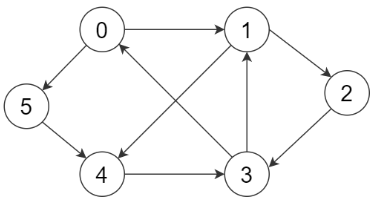
\includegraphics[height=0.6\textheight]{figures/eulerian_path_example.png}
        \caption{Một đồ thị có đường đi Euler $0 \rightarrow 1 \rightarrow 2 \rightarrow 3 \rightarrow 0 \rightarrow 5 \rightarrow 4 \rightarrow 3 \rightarrow 1 \rightarrow 4$}
    \end{figure}
\end{frame}

\section{Giải trình tự và lắp ráp các đoạn DNA}

\begin{frame}{Cấu trúc của một chuỗi DNA}
    \begin{columns}
        \begin{column}{0.47\textwidth}
            Tất cả các đoạn DNA bao gồm bốn loại ba-zơ tạo nên: Adenine (A), Thymine (T), Guanine (G) và Cystosine (C).

            Cấu hình của toàn bộ bộ gen dựa trên một loạt các chuỗi được đọc từ bộ gen đó.

            Một chuỗi DNA đầy đủ bao gồm hàng triệu nucleotide nên không có cách nào để nắm được toàn bộ cấu trúc một cách rõ ràng.
        \end{column}
        \begin{column}{0.47\textwidth}
            \begin{figure}[h!]
                \centering
                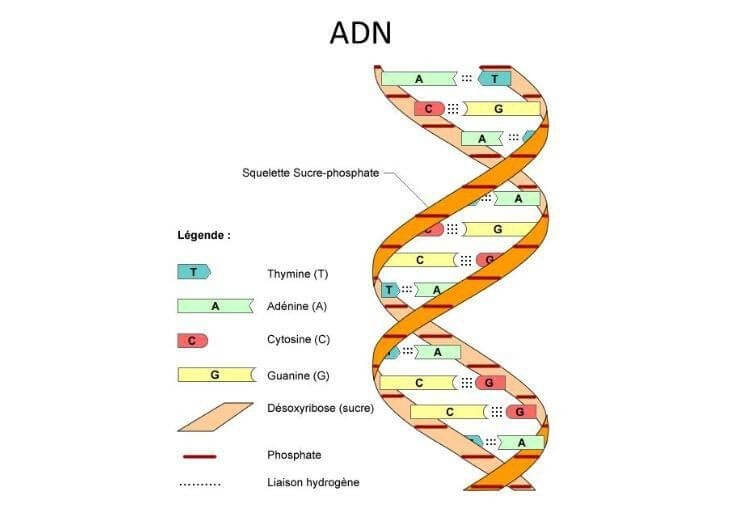
\includegraphics[height=0.75\textheight]{figures/dna_strands_example.jpg}
                \caption{Hình ảnh minh họa một DNA}
            \end{figure}
        \end{column}
    \end{columns}
        
        
\end{frame}


\begin{frame}{Các công trình liên quan giải trình tự DNA}

    \begin{columns}
        \begin{column}{0.47\textwidth}
            Quá trình giải trình tự DNA là thu được một loạt các đoạn DNA (Reads) và công việc là xây dựng lại chuỗi DNA ban đầu.

            Do một chuỗi DNA đầy đủ có độ dài lên đến hàng tỷ nucleotide nên không có cách nào đọc được toàn bộ chuỗi DNA ban đầu.

            Ta chỉ có thể đọc được các đoạn DNA ngắn từ 500 đến 1200 nucleotide.
        \end{column}
        \begin{column}{0.47\textwidth}
            \begin{figure}[h!]
                \centering
                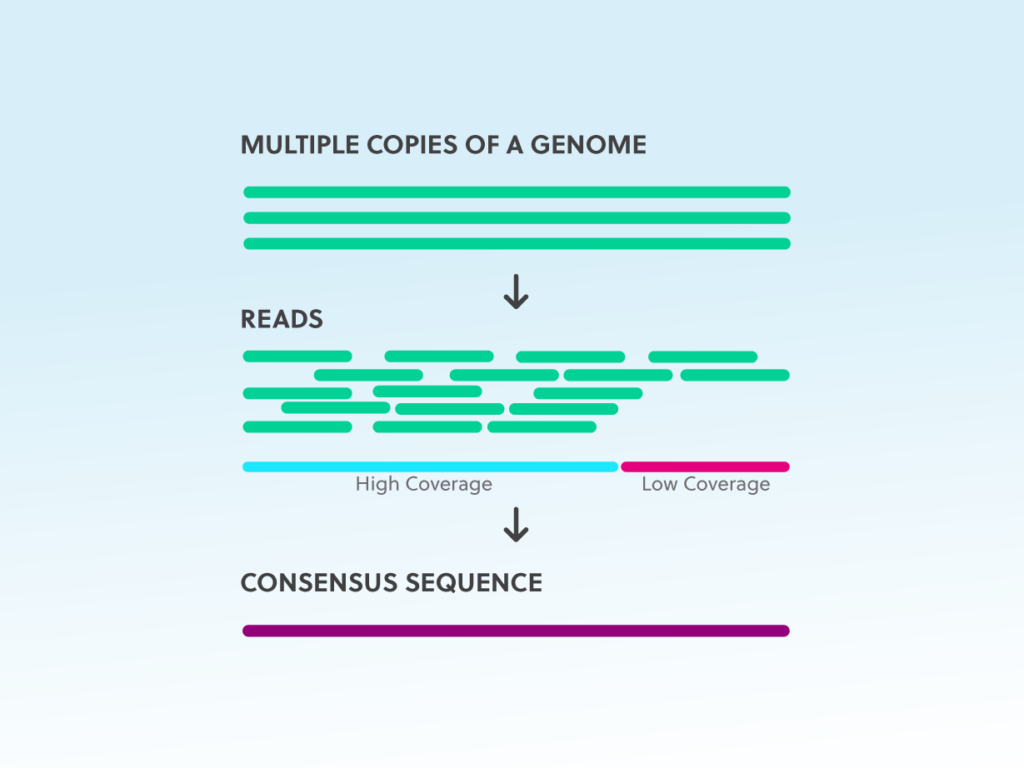
\includegraphics[height=0.75\textheight]{figures/dna_reads_example.png}
                \caption{Minh họa quá trình đọc một chuỗi DNA}
            \end{figure}
        \end{column}
    \end{columns}
    
\end{frame}

\begin{frame}{Những khó khăn trong quá trình lắp ráp}
    Tỷ lệ sai này khoảng 1 \% đến 3 \% của DNA do máy giải trình tự tạo ra

    Chuỗi DNA có cấu trúc xoắn kép.

    Bộ gen của sinh vật nói chung có một lượng lớn các chuỗi lặp đi lặp lại nhiều lần.

    Ví dụ, ta xét một bộ gen cụ thể có chuỗi lặp lại có độ dài 2000 nucleotide. Hiện nay không có một máy giải trình tự nào có thể đọc được một đoạn DNA co độ dài như vậy, vì vậy không có cách nào để đọc toàn bộ đoạn lặp lại.

\end{frame}

\begin{frame}{Phương pháp tiếp cận lý thuyết đồ thị giải trình tự DNA}


    Các công trình trước đây thường dựa trên cách tiếp cận "overlap-layout-concensus".

    \cite{idury1995new} đã đề xuất giải trình tự bằng cách xây dựng đồ thị có hướng, tìm đường đi Euler trong đồ thị.

    Cụ thể, \cite{idury1995new} sử dụng de Bruijn dựa trên các đoạn DNA có đội dài là $k$ (một số tài liệu gọi là k-mers).
    Các đỉnh được gán nhãn bởi các đoạn DNA có độ dài là $k-1$, các cạnh được gán nhãn bởi các đoạn DNA có độ dài là $k$.
\end{frame}

\begin{frame}{Phương pháp tiếp cận lý thuyết đồ thị giải trình tự DNA}

    Để giải trình tự DNA, ta tìm đường đi Euler trong đồ thị de Bruijn xây dựng được.

    Do một đồ thị có hướng có thể có nhiều đường đi Euler, ta quan tâm đến các phép biến đổi đồ thị sao cho đường đi Euler thu được biểu diễn chuỗi DNA thực sự ban đầu.

    
\end{frame}

\section{Xây dựng chuỗi DNA với đồ thị de Bruijn}

\begin{frame}{Đồ thị de Bruijn}
    Đồ thị de Bruijn là một đồ thị có hướng với các đỉnh biểu diễn các chuỗi ký tự từ bảng chữ cái và các cạnh được biểu diễn bắt đầu bằng chuỗi biểu diễn đỉnh bắt đầu và kết thúc bằng chuỗi biểu diễn đỉnh kết thúc.

    Việc xây dựng đồ thị này phụ thuộc vào một tập các mảnh hoặc các đoạn có độ dài $k$ từ dãy cụ thể hiện có.

    Mỗi đỉnh được gán nhãn bởi một đoạn có chiều dài $k-1$ và cạnh có hướng tồn tại giữa hai đỉnh đại diện cho một trong đoạn có chiều dài $k$.

    $k-1$ ký tự trong đoạn biểu diễn đỉnh bắt đầu cạnh và tương tự, $k-1$ ký tự cuối cùng biểu diễn đỉnh nhận.

\end{frame}


\begin{frame}{Đồ thị de Bruijn}
    \begin{figure}[h!]
        \centering
        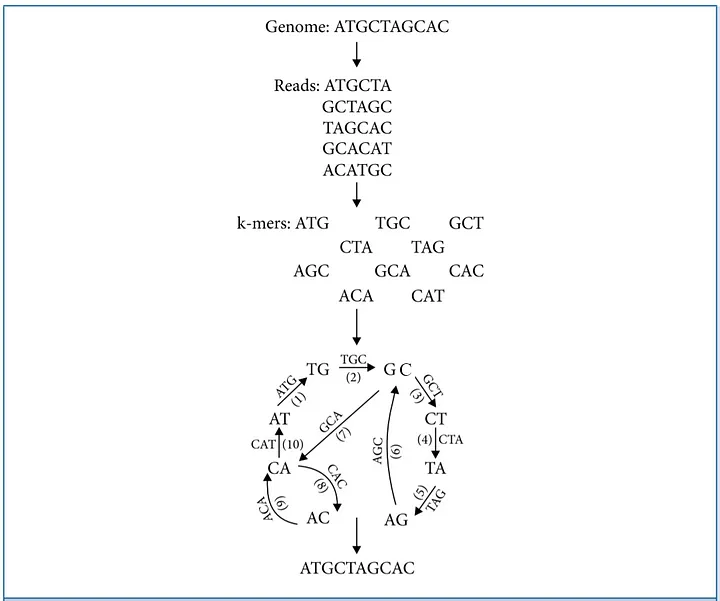
\includegraphics[height=0.75\textheight]{figures/de_Bruijn_graph_from_short_read_example.png}
        \caption{Ví dụ đồ thị de Bruijn được tạo từ các Reads}
    \end{figure}
\end{frame}

\begin{frame}{Đồ thị de Bruijn}
    \begin{figure}[h!]
        \centering
        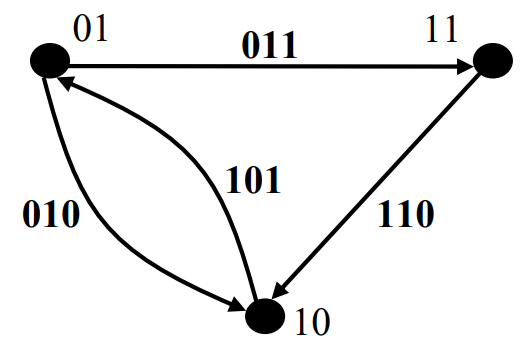
\includegraphics[width=0.35\textwidth]{1.png}
        \caption{Một đồ thị de Bruijn cho chuỗi "0110101" với các đoạn chiều dài là 3.}
        \label{fig:1}
    \end{figure}

    Ví dụ, ta xây dựng một đồ thị de Bruijn cho chuỗi "0110101" sử dụng các đoạn có độ dài $k=3$.

    Bốn bộ ba có mặt trong chuỗi là 011, 110, 101 (xuất hiện hai lần) và 010.
    
    Hình \ref{fig:1} cho thấy đồ thị de Bruijn trùng với chuỗi này.
\end{frame}


\begin{frame}
    \begin{figure}[h!]
        \centering
        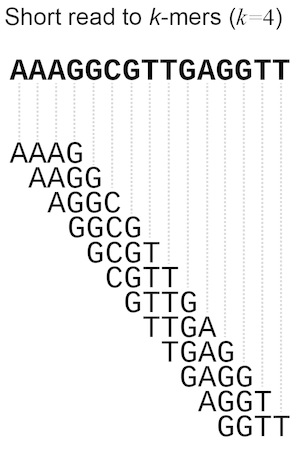
\includegraphics[width=0.4\textwidth]{de_Bruijn_graph_example.png}
        \caption{Các k-mers được tạo từ một chuỗi các nucleotide}
    \end{figure}
\end{frame}
    
\begin{frame}
    \begin{figure}[h!]
        \centering
        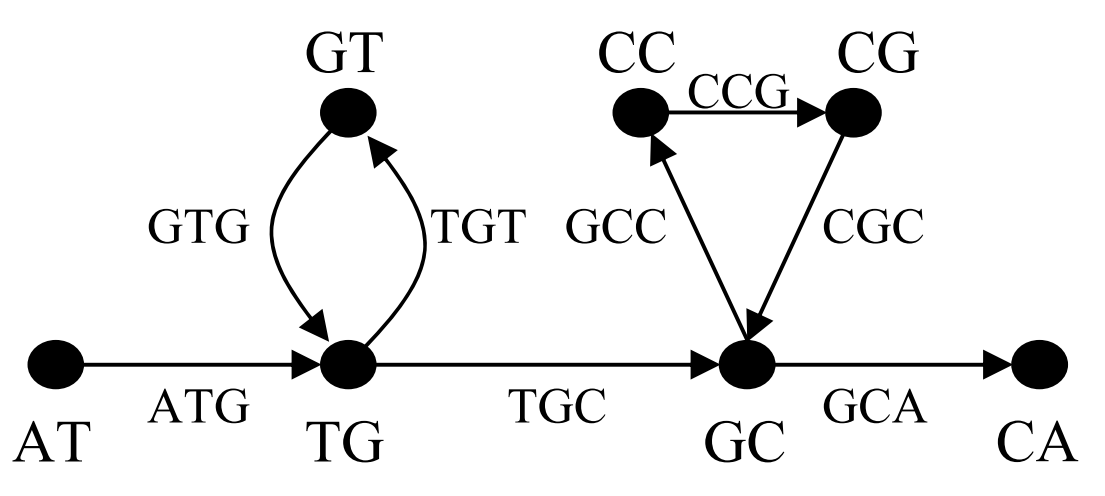
\includegraphics[width=0.6\textwidth]{2.png}
        \caption{Một đồ thị de Bruijn cho chuỗi ATGTGCCGCA.}
        \label{fig:2}
    \end{figure}

    Hình \ref{fig:2} minh họa một đồ thị de Bruijn cho một chuỗi đơn giản ATGTGCCGCA.

    Các đỉnh được đánh dấu bằng các đoạn có độ dài là 2 và các cạnh được đánh dấu bằng các đoạn có độ dài là 3, biểu diễn cho các bộ ba thu được từ chuỗi ban đầu.
\end{frame}

\begin{frame}
    \begin{figure}[h!]
        \centering
        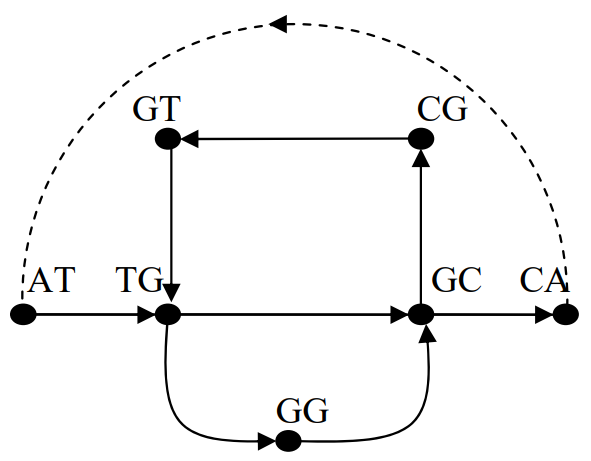
\includegraphics[width=0.5\textwidth]{3.png}
        \caption{Một đồ thị được xây dựng từ tập các đoạn đọc được $S$}
        \label{fig:3}
    \end{figure}

    Với tập hợp các đoạn $S = \lbrace ATG, TGG, TGC, GTG, GGC, GCA, GCG, CGT \rbrace$,
    đồ thị sẽ có các đỉnh được gán nhãn bởi các đoạn có độ dài là 2 và các cạnh được gán nhãn bởi các đoạn có độ dài là 3.

\end{frame}

\begin{frame}
    Có hai đường đi Euler khác nhau cho toàn bộ đồ thị, tạo ra các chuỗi ATGGCGTGCA và ATGCGTGGCA.

    Phương pháp tiếp cận lắp ráp các đoạn DNA này được một số nà nghiên cứu gọi là phương pháp đường đi Euler, tạo ra một bài toán về xác suất.

    Ta thấy với tập hợp mảnh đã cho ta có thể xây dựng hai chuỗi khác nhau dựa trên việc có hai đường đi Euler khác nhau.

    Tổng quát hơn, khi ta được cung cấp dữ liệu đầy đủ và không có lỗi, ta có thể thấy rằng xác suất tái tạo lại chuỗi DNA ban đầu với một tập hợp các đoạn là:

    \begin{equation}
        \dfrac{1}{\text{tổng số chu trình/đường đi Euler trong đồ thị de Bruijn}}
    \end{equation}
\end{frame}

\section{Định lý BEST}

\begin{frame}{Định lý BEST}
    \begin{dl}[Định lý BEST]
        Cho một đồ thị có hướng liên thông $G$ và tập các đỉnh $V(G)=\lbrace v_1, v_2, \dots, v_n \rbrace$ tất cả đều có bậc vào bằng bậc ra, số chu trình Euler là $\lvert s(G) \rvert$ được tính theo công thức sau, với $\lvert t_i (G) \rvert$ là số cây khung hướng đến gốc là một đỉnh $v_i$ bất kỳ trong $G$:

        \begin{equation*}
            \lvert s(G) \rvert = \lvert t_i (G) \rvert \prod_{j=1}^n \big( d^+ (v_j) - 1 \big)!
        \end{equation*}
    \end{dl}
\end{frame}

\begin{frame}{Ma trận kề}
    Một ma trận là ma trận kề, liệt kê số các cạnh giữa các đỉnh trong đồ thị.

    Ma trận này có kích thước $n \times n$ với $n$ là số đỉnh của đồ thị $G$.

    Nếu $a_{ij}$ là số cạnh có hướng rời đỉnh $v_i$ và đi vào đỉnh $v_j$ trong đồ thị $G$, khi đó $a_{ij}$ là phần tử $i, j$ của ma trận.

\end{frame}

\begin{frame}{Ma trận kề}
    \begin{figure}[h!]
        \centering
        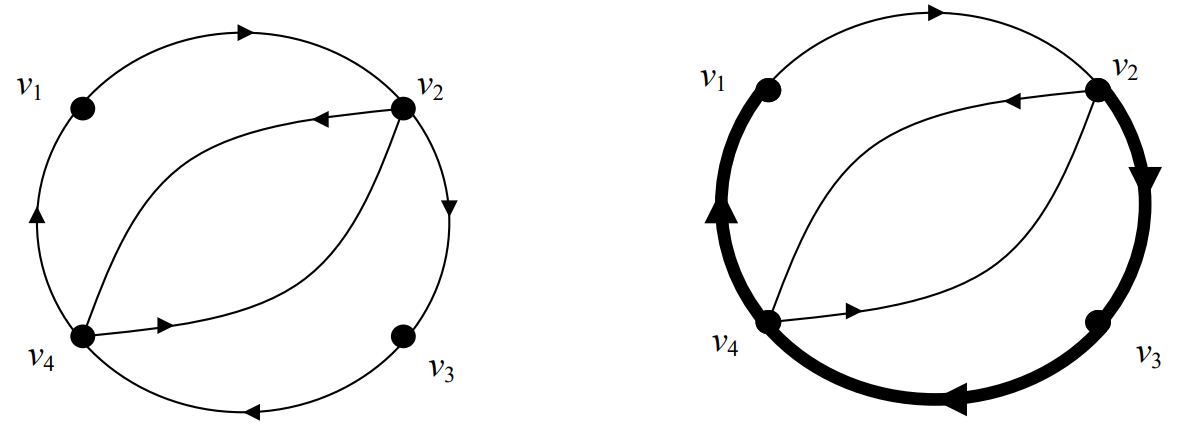
\includegraphics[width=0.6\textwidth]{4.png}
        \caption{Sử dụng chu trình Euler $v_1 v_2 v_4 v_2 v_3 v_4 v_1$ trong đồ thị $G$, ánh xạ tạo ra cây khung hướng đến đỉnh $v_1$ biểu thị trong các đường đậm trong đồ thị bên phải.}
        \label{fig:4}
    \end{figure}
\end{frame}

\begin{frame}{Ma trận kề}
    Ma trận kề của đồ thị được ký hiệu là $A(G)$ của đồ thị $G$ từ hình \ref{fig:4}.

    \begin{equation*}
        A(G) = \begin{pmatrix}
            0 & 1 & 0 & 0 \\ 
            0 & 0 & 1 & 1 \\ 
            0 & 0 & 0 & 1 \\ 
            1 & 1 & 0 & 0
        \end{pmatrix}
    \end{equation*}
\end{frame}

\begin{frame}{Ma trận đường chéo}

    Ma trận thứ hai có thể được xây dựng từ một đồ thị là một ma trận đường chéo.

    Ma trận này điền các bậc vào của từng đỉnh trong đồ thị vào đường chéo.

    Tất cả các phần tử khác là 0.

    Sử dụng cùng đồ thị $G$ ở trên, ma trận đường chéo $D(G)$ là:

    \begin{equation*}
        D(G) = \begin{pmatrix}
            1 & 0 & 0 & 0 \\
            0 & 2 & 0 & 0 \\
            0 & 0 & 1 & 0 \\
            0 & 0 & 0 & 2
        \end{pmatrix}
    \end{equation*} 
    
\end{frame}

\begin{frame}{Ma trận Laplace}

    Ma trận này là kết quả của $D(G)$ trừ $A(G)$.

    \begin{equation*}
        L(G) = \begin{pmatrix}
            1 & -1 & 0 & 0 \\
            0 & 2 & -1 & -1 \\
            0 & 0 & 1 & -1 \\
            -1 & -1 & 0 & 2 \\
        \end{pmatrix}
    \end{equation*}

    Tính định thức của ma trận bằng cách bỏ đi hàng $i$ và cột $i$ bất kỳ ta thu được giá trị $k=2$.

    Hơn nữa, nếu ta tính cả ba phần phụ đại số còn lại của $L(G)$, ta có thể thấy tất cả đều bằng 2.

    Lý do từ việc là tổng tất cả các hàng và cột đều bằng 0 và sẽ đúng cho tất cả các ma trận có tổng các hàng và cột đều bằng 0.
    Chứng minh được nêu trong \cite{fleischner1990eulerian}.
\end{frame}

\begin{frame}{Định lý cây ma trận}
    \begin{dl}[Định lý cây ma trận]
        Cho một đồ thị có hướng $G$ với tập các đỉnh $V(G)=\lbrace v_1, v_2, \dots, v_n \rbrace$ và một tập các cây khung $t_i (G)$ hướng đến đỉnh $v_i$ và $\lvert t_i(G) \rvert$ bằng với phần phụ đại số của ma trận $L(G)$ trên hàng và cột thứ $i$:

        \begin{equation*}
            \lvert t_i(G) \rvert = \det_{i, i} L(G)
        \end{equation*}
    \end{dl}
\end{frame}

\section{Bài toán siêu đường đi Euler}

\begin{frame}{Định nghĩa bài toán siêu đường đi Euler}

    Cho một tập các Read $\mathcal{P} = \lbrace P_1, P_2, \dots, P_n \rbrace$ (hay còn gọi là các đường đi).
    Từ các Read này, ta xây dựng một đồ thị de Bruijn $G$.


    Bài toán (siêu) đường đi Euler (được gọi ở đây là ESP) nhằm thực hiện những điều sau:
    Cho một đồ thị Euler $G$ với một tập các đường đi $P$ (trong các tài liệu khác còn gọi là tập các Read) trong đồ thị, tìm một đường đi Euler trong đồ thị $G$ chứa tất cả các thành phần của $P$ là đường đi con.
\end{frame}

\begin{frame}{Ví dụ}

    Giả sử ta có các đoạn sau: (1) $ATGG$, (2) $TGGCG$, (3) $GGCGTG$ và (4) $CGTGCA$.

    Hình \ref{fig:3} biểu diễn đồ thị de Bruijn xây dựng từ các đoạn trên.

    Có hai đường đi Euler khác nhau cho toàn bộ đồ thị, tạo ra các chuỗi ATGGCGTGCA và ATGCGTGGCA.

    Nhưng chỉ có chuỗi ATGGCGTGCA chứa tất cả các đoạn đọc được.

    
\end{frame}

\begin{frame}{Cách tiếp cận}
    Ta duy trì sự tương đương giữa đồ thị $G$ và hệ thống của các đường đi $P$ bằng một loạt các phép biến đổi $(G, P) \rightarrow (G_1, P_1) \rightarrow \dots \rightarrow (G_k, P_k)$.

    Tập kết quả $(G_k, P_k)$ là một biểu diễn gọn hơn nhiều của $(G, P)$.
    
\end{frame}

\begin{frame}{Phép tách rời $x, y$}
    \begin{columns}
        
    
    \begin{column}{0.47\textwidth}
        
    
    Có thể được thực hiện trong trường hợp cạnh không có bội số trong đồ thị $G$ đã cho.
    
    Nếu ta có hai cạnh kề nhau $x$ và $y$ trong đồ thị $G$ và ba tập Read đủ từ $\mathcal{P}$, một trong số đó có cả hai cạnh liên tiếp, một tập kết thúc với $x$ và một bắt đầu với $y$, phép tách này được thực hiện. Cụ thể, đỉnh nối với hai cạnh bị kéo ra xa, tạo ra một cạnh mới $z$.

    \end{column}

    \begin{column}{0.47\textwidth}
        

    \begin{figure}[h!]
        \centering
        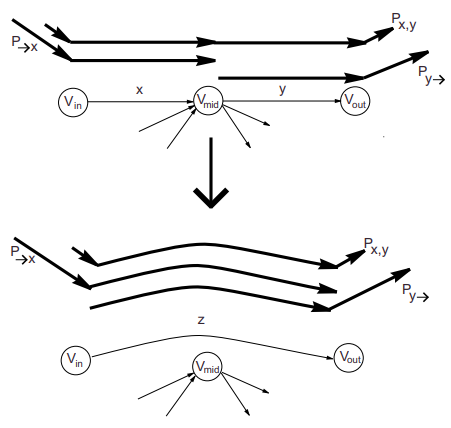
\includegraphics[height=0.7\textheight]{figures/xy_detachment.png}
        \caption{Minh họa phép tách rời $x, y$ \cite{pevzner2001new}}
    \end{figure}

    \end{column}


    \end{columns}
\end{frame}

\begin{frame}{Phép tách rời $x, y$}
    \begin{figure}[h!]
        \centering
        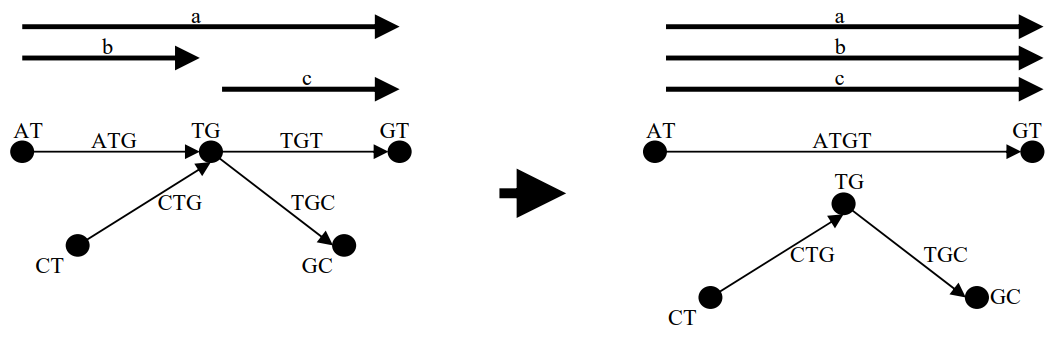
\includegraphics[width=0.9\textwidth]{6.png}
        \caption{Một phép tách rời $x, y$ kết nối các cạnh $ATG$ và $TGT$.}
        \label{fig:6}
    \end{figure}
\end{frame}

\begin{frame}{Phép tách rời $x, y_1$}
    Giống như phép tách rời trước đó, phép tách rời $x, y_1$ tương tự phụ thuộc vào tập các Read.

    Tập đầu tiên là tất cả các đường dẫn chứa một bản sao của cạnh có bội số $x$ theo sau là $y_1$.

    Tập thứ hai và thứ ba là những tập kết thúc với cạnh có bội số $x$ và những tập bắt đầu bằng cạnh $y_1$.

    \begin{figure}[h!]
        \centering
        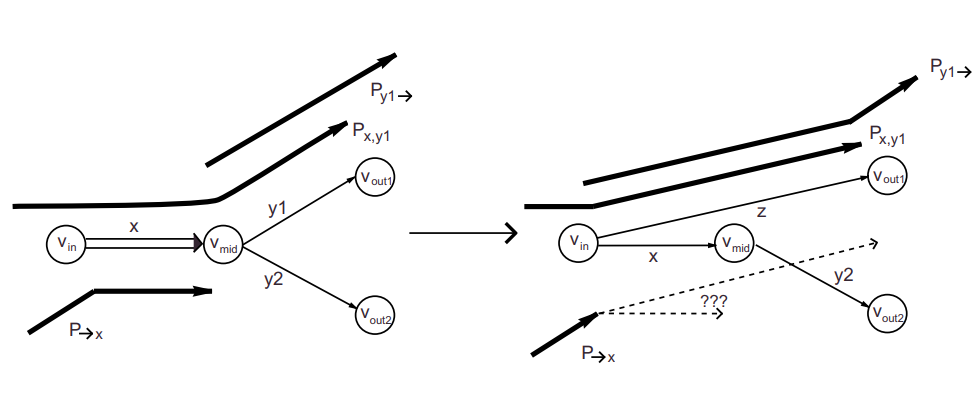
\includegraphics[width=0.6\textwidth]{figures/xy1_detachment.png}
        \caption{Minh họa phép tách rời $x, y_1$ \cite{pevzner2001new}}
    \end{figure}
\end{frame}

\begin{frame}{Phép tách rời $x, y_1$}
    Nếu không có đường đi nào kết thúc trên $x$ thì ta có thể xóa một bản sao của $x$ một cách an toàn và tạo một cạnh mới $xy_1$.

    \begin{figure}[h!]
        \centering
        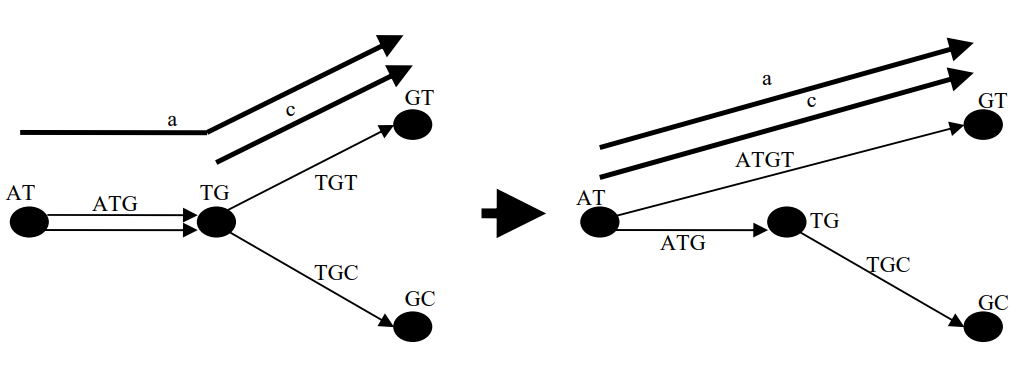
\includegraphics[width=0.9\textwidth]{7.png}
        \caption{Một phép tách rời $x, y_1$ thành công tại cạnh đa $ATG$.}
        \label{fig:7}
    \end{figure}
\end{frame}

\begin{frame}{Ví dụ}

    \begin{columns}
        \begin{column}{0.47\textwidth}
            Giả sử ta có các đoạn sau: (1) $ATGG$, (2) $TGGCG$, (3) $GGCGTG$ và (4) $CGTGCA$.

        Với những đoạn này, có hai phép tách rời cạnh đơn quan trọng ta có thể thực hiện và vẫn duy gì sự tương đương với đồ thị ban đầu.

        Phép biến đổi này được thể hiện trong hình \ref{fig:8}.
        \end{column}
        \begin{column}{0.47\textwidth}
            \begin{figure}[h!]
                \centering
                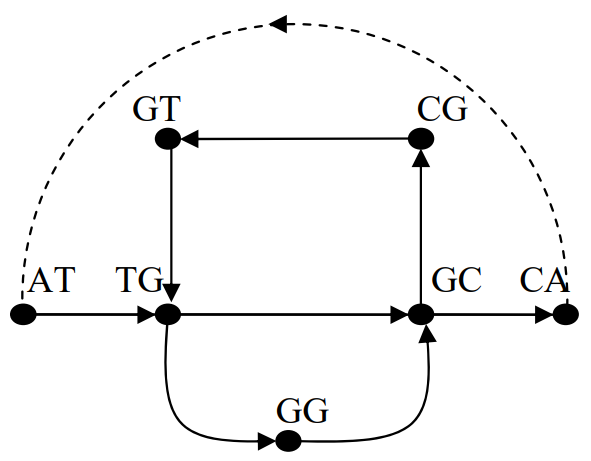
\includegraphics[height=0.6\textheight]{3.png}
                \caption{Một đồ thị được xây dựng từ tập các đoạn đọc được $S$}
                \label{fig:3}
            \end{figure}
        \end{column}
    \end{columns}

    
\end{frame}

\begin{frame}{Ví dụ}
    \begin{columns}
        \begin{column}{0.47\textwidth}
            Phép tách đầu tiên diễn ra tại đỉnh $TG$. Đoạn (1) đi từ $AT$ đến $GG$ qua đỉnh $TG$, trong khi các đoạn (3) và (4) đi qua $TG$ từ $GT$ rồi chuyển sang $GC$.

            Phép tách quan trọng thứ hai diễn ra tại đỉnh $GC$. Tại đây, cả đoạn (2) và (3) đều đi qua $GC$ từ $GG$ rồi đến $CG$. 
            Hơn nữa, đoạn (4) đi qua $GC$ sau khi từ $TG$ và kết thúc tại $CA$.
        \end{column}
        \begin{column}{0.47\textwidth}
            \begin{figure}[h!]
                \centering
                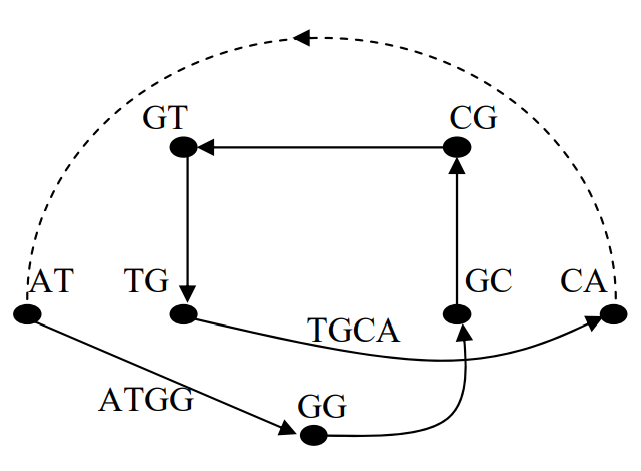
\includegraphics[height=0.6\textheight]{8.png}
                \caption{Đồ thị được tạo ra sau hai phép tách rời trên đồ thị trong hình \ref{fig:3}.}
                \label{fig:8}
            \end{figure}
        \end{column}
    \end{columns}
\end{frame}

\section{Giải trình tự DNA với Nanopore}

\begin{frame}{Giải trình tự DNA với Nanopore}
    Nanopore là một thiết bị có đường kính vài nguyên tử với hy vọng có thể đọc cả một đoạn DNA đầy đủ hoạt động theo cơ chế điện học.

    Video minh họa: \url{https://www.youtube.com/watch?v=E9-Rm5AoZGw}
\end{frame}

\begin{frame}{Giải trình tự DNA với Nanopore}
    \begin{figure}
        \centering
        \begin{minipage}{.45\textwidth}
        \centering
        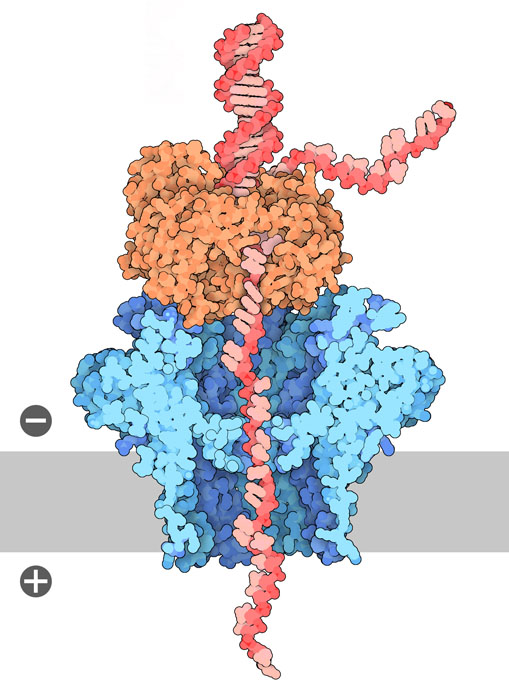
\includegraphics[width=.75\linewidth]{figures/nanopore_1.jpg}
        \end{minipage}
        \begin{minipage}{.45\textwidth}
        \centering
        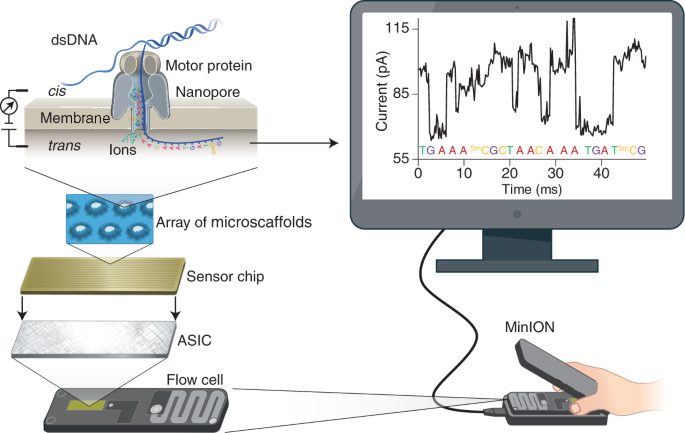
\includegraphics[width=.75\linewidth]{figures/nanopore_2.png}
        \end{minipage}
        \caption{Minh họa Nanopore}
    \end{figure}
\end{frame}

\begin{frame}{Giải trình tự DNA với Nanopore}

    Ưu điểm:

    \begin{itemize}
        \item Đọc được một đoạn dài hơn rất nhiều so với phương pháp trước đây, có hy vọng sẽ đọc được toàn bộ chuỗi DNA.
    \end{itemize}

    Nhược điểm:

    \begin{itemize}
        \item Thực tế thì mỗi đoạn DNA đọc được chỉ dài khoảng 100000 nucleotide.
        \item Quá trình đọc có lỗi.
        \item Khó xác định là chuỗi bên gốc hay bên kia trong chuỗi xoắn kép được đọc.
        \item Chiều đọc có thể bị ngược nhau trong các lần đọc.
    \end{itemize}
    
\end{frame}

\section{Thực nghiệm}

\begin{frame}{Minh họa quá trình giải trình tự}
    \begin{figure}[h!]
        \centering
        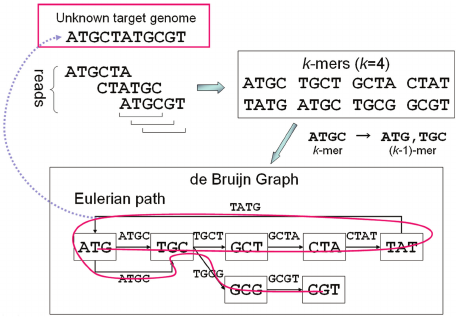
\includegraphics[width=0.75\textwidth]{Illustration-of-de-Bruijn-graph-based-assembly.png}
        \caption{Minh họa quá trình giải trình tự}
    \end{figure}
\end{frame}


\begin{frame}{Giả thiết}
    \begin{itemize}
        \item Các đoạn Reads đọc được không có lỗi
        \item Các Read đều đến từ một bên của chuỗi DNA ban đầu
        \item Mỗi một Read sẽ có đoạn giao đủ dài với một vài Read khác
    \end{itemize}
\end{frame}

\begin{frame}
    \begin{figure}[h!]
        \centering
        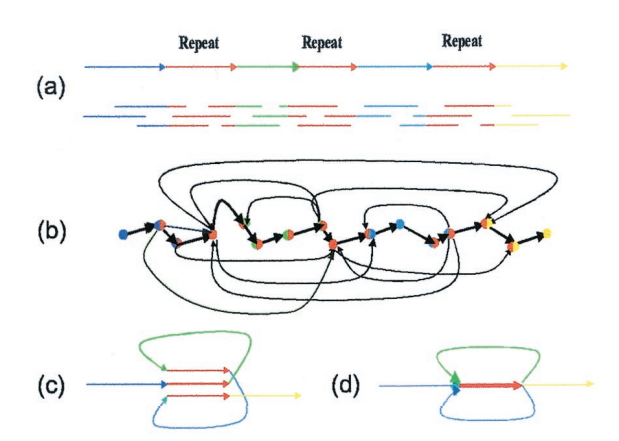
\includegraphics[width=0.75\textwidth]{figures/de_Bruijn_graph_with_repeat_1.png}
        \caption{Minh họa đồ thị de Bruijn có các đoạn lặp lại}
    \end{figure}
\end{frame}

\begin{frame}
    \begin{figure}[h!]
        \centering
        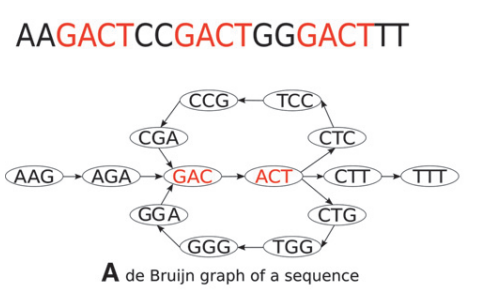
\includegraphics[width=0.75\textwidth]{figures/de_Bruijn_graph_with_repeat_2.png}
        \caption{Minh họa đồ thị de Bruijn có các đoạn lặp lại}
    \end{figure}
\end{frame}

\begin{frame}{Các bước thực hiện chính}
    \begin{enumerate}
        \item Đọc các Read (định dạng .fastq)
        \item Tiền xử lý, xác định các khoảng chồng lấn giữa các Read (quan trọng)
        \item Xây dựng đồ thị de Bruijn và xác định bội số của các cạnh
        \item Kiểm tra đồ thị có phải đồ thị Euler không
        \item Thực hiện bài toán siêu đường đi Euler
        \item Kiểm tra đồ thị mới có phải đồ thị Euler không
        \item Tính số đường đi Euler có thể
        \item Tìm đường đi Euler và dãy DNA gốc
    \end{enumerate}
    
\end{frame}

\begin{frame}{Chiến lược giải bài toán siêu đường đi Euler}
    Chia làm 2 giai đoạn tách biệt:

    \begin{enumerate}
        \item Chỉ gộp các cạnh đơn với nhau và các các cạnh bội cùng bội số tại một đỉnh chỉ có duy nhất một cạnh vào và một cạnh ra.
        \item Thực hiện gộp các cạnh có khác bội số và các cạnh đơn phát sinh.
    \end{enumerate}
\end{frame}


\begin{frame}{Thủ tục chương trình chính}
    \begin{algorithm}[H]
        \DontPrintSemicolon
        \KwIn{seqs: \KwSty{List[str]}, k: \KwSty{int}}
        INIT\_DE\_BRUIJN\_GRAPH(seqs=seqs, k=k)\;
        IS\_EULERIAN()\;
        MERGE\_EQUAL\_MULTIPLICITIES\_EDGES()\;
        MERGE\_UNEQUAL\_MULTIPLICITIES\_EDGES()\;
        \If{IS\_EULERIAN()} {
            GET\_NUMBERS\_EULERIAN\_PATH()\;
            FIND\_EULERIAN\_PATH()\;
        }
        
        \caption{MAIN}
    \end{algorithm}
    
\end{frame}

\begin{frame}{Thuật toán khởi tạo đồ thị de Bruijn}
    \begingroup
        \scalebox{0.3}{
            \begin{minipage}{1.8\linewidth}
                \begin{algorithm}[H]
                    \DontPrintSemicolon
                    \KwIn{seqs: \KwSty{List[str]}, k: \KwSty{int}}

                    vertex\_list: \KwSty{List[Vertex]} $\gets \emptyset$\;
                    vertex\_dict: \KwSty{Dict[str, Vertex]} $\gets \lbrace \rbrace$\;
                    edge\_list: \KwSty{List[Edge]} $\gets \emptyset$\;
                    edge\_dict: \KwSty{Dict[str, Edge]} $\gets \lbrace\rbrace$\;
                    read\_list: \KwSty{List[Read]} $\gets \emptyset$\;

                    \For{s $\gets$ 0 \KwTo seqs.length}{
                        seq: \KwSty{str} $\gets$ seqs[s]\;
                        read: \KwSty{Read} $\gets$ Read(sequence=seq, read\_id=s)\;
                        read\_list.add(read)\; 
                    }
                    align\_read(min\_length=k)\;
                    \ForEach{read $\in$ read\_list}{
                        seq: \KwSty{str} $\gets$ read.sequence\;

                        \For{i $\gets$ 0 \KwTo seq.length - k + 1}{
                            k\_mer: \KwSty{str} $\gets$ seq[i:i+k]\;
                            prefix: \KwSty{str} $\gets$ k\_mer[:k-1]\;
                            suffix: \KwSty{str} $\gets$ k\_mer[1:]\;

                            \If{prefix $\in$ vertex\_dict} {
                                p\_vertex: \KwSty{Vertex} $\gets$ vertex\_dict[prefix]\;
                            } \Else{
                                p\_vertex: \KwSty{Vertex} $\gets$ new\_vertex(sequence=prefix)\;
                            }

                            \If{suffix $\in$ vertex\_dict} {
                                s\_vertex: \KwSty{Vertex} $\gets$ vertex\_dict[suffix]\;
                            } \Else{
                                s\_vertex: \KwSty{Vertex} $\gets$ new\_vertex(sequence=suffix)\;
                            }
                            \If{k\_mer $\in$ edge\_dict} {
                                edge: \KwSty{Edge} $\gets$ edge\_dict[k\_mer]\;
                                determine\_edge\_multiplicities(read=read, edge=edge, i=i)\;
                            } \Else {
                                edge: \KwSty{Edge} $\gets$ new\_edge(in\_vertex=p\_vertex, out\_vertex=s\_vertex, sequence=k\_mer)\;
                            }
                            \If{edge $\notin$ read.edges} {
                                read.edges.add(edge)\;
                            }
                            \If{read $\notin$ edge.reads}{
                                edge.reads.add(read)\;
                            }                            
                            \If{read $\notin$ edge.position\_in\_read} {
                                edge.position\_in\_read[read] $\gets$ [i]\;
                            } \Else{
                                edge.position\_in\_read[read].add(i)\;
                            }
                            \If{edge $\notin$ read.edge\_to\_positions} {
                                read.edge\_to\_positions[edge] $\gets$ [i]\;
                            } \Else{
                                read.edge\_to\_positions[edge].add(i)\;
                            }
                            read.position\_to\_edge[i] $\gets$ edge\;
                        }
                    }
                    \caption{INIT\_DE\_BRUIJN\_GRAPH}
                \end{algorithm}
            \end{minipage}
        }
    \endgroup
\end{frame}

\begin{frame}{Thuật toán kiểm tra hai cạnh cùng bội có thể merge được không}
    \begingroup
        \scalebox{0.45}{
            \begin{minipage}{1.8\linewidth}
                \begin{algorithm}[H]
                    \DontPrintSemicolon
                    \KwIn{graph: \KwSty{Graph}, vertex\_list: \KwSty{List[Vertex]}}
                    \While{vertex\_list.length > 0}{
                        vertex: \KwSty{int} $\gets$ vertex\_list.pop(0)\;
                        num\_in\_edge: \KwSty{int} $\gets$ vertex.in\_edges.length\;
                        num\_out\_edge: \KwSty{int} $\gets$ vertex.out\_edges.length\;

                        \If{abs(vertex.compute\_degree()) = 1} {
                            continue\;
                        }

                        \If{num\_in\_edge = 0 $\cap$ num\_out\_edge = 0} {
                            continue\;
                        }

                        in\_edges: \KwSty{List[Edge]} = vertex.in\_edges.copy()\;
                        out\_edges: \KwSty{List[Edge]} = vertex.out\_edges.copy()\;

                        \If{num\_in\_edge = num\_out\_edge} {
                            \ForEach{x $\in$ in\_edges}{
                                x\_reads $\gets$ x.reads.copy()\;
                                \ForEach{y $\in$ out\_edges} {
                                    \If{x.multiplicities = y.multiplicities} {
                                        \For{read $\in$ x\_reads} {
                                            \If{read $\in$ y.reads} {
                                                \If{read.check\_consecutive\_edges(x=x, y=y)} {
                                                    \If{graph.merge(x=x, y=y)} {
                                                        graph.clean()\;
                                                    }
                                                }
                                            }
                                        }
                                    }
                                }
                            }
                        }
                    }
                    graph.clean()
                    \caption{MERGE\_EQUAL\_MULTIPLICITIES\_EDGES}
                \end{algorithm}
            \end{minipage}
        }
    \endgroup
\end{frame}


\begin{frame}{Thuật toán kiểm tra hai cạnh khác bội có thể merge được không}
    \begingroup
        \scalebox{0.45}{
            \begin{minipage}{1.8\linewidth}
                \begin{algorithm}[H]
                    \DontPrintSemicolon
                    \KwIn{graph: \KwSty{Graph}, vertex\_list: \KwSty{List[Vertex]}}
                    \While{vertex\_list.length > 0}{
                        vertex: \KwSty{int} $\gets$ vertex\_list.pop(0)\;
                        num\_in\_edge: \KwSty{int} $\gets$ vertex.in\_edges.length\;
                        num\_out\_edge: \KwSty{int} $\gets$ vertex.out\_edges.length\;

                        \If{abs(vertex.compute\_degree()) = 1} {
                            continue\;
                        }

                        \If{num\_in\_edge = 0 $\cap$ num\_out\_edge = 0} {
                            continue\;
                        }

                        in\_edges: \KwSty{List[Edge]} = vertex.in\_edges.copy()\;
                        out\_edges: \KwSty{List[Edge]} = vertex.out\_edges.copy()\;

                        \If{num\_in\_edge = num\_out\_edge} {
                            \ForEach{x $\in$ in\_edges}{
                                x\_reads $\gets$ x.reads.copy()\;
                                \ForEach{y $\in$ out\_edges} {
                                    \If{x.multiplicities = y.multiplicities} {
                                        \For{read $\in$ x\_reads} {
                                            \If{read $\in$ y.reads} {
                                                \If{read.check\_consecutive\_edges(x=x, y=y)} {
                                                    \If{graph.merge\_mul(x=x, y=y)} {
                                                        graph.clean()\;
                                                    }
                                                }
                                            }
                                        }
                                    }
                                }
                            }
                        }
                    }
                    graph.clean()
                    \caption{MERGE\_UNEQUAL\_MULTIPLICITIES\_EDGES}
                \end{algorithm}
            \end{minipage}
        }
    \endgroup
\end{frame}

\begin{frame}{Thuật toán kiểm tra đồ thị Euler}
    \begingroup
        \scalebox{0.8}{
            \begin{minipage}{1.5\linewidth}
                \begin{algorithm}[H]
                    \DontPrintSemicolon
                    \KwIn{vertex\_list: \KwSty{List [Vertex]}}
                    diff\_list: \KwSty{List [int]} $\gets \emptyset$\;
                    \ForEach{vertex $\in$ vertex\_list}{
                        diff\_mul $\gets$ vertex.compute\_degree()\;
                        \If{diff\_mul = 0} {
                            continue\;
                        } \Else {
                            \If{$\lvert$ diff\_mul $\rvert \geq$ 2} {
                                \Return{false}\;
                            }
                            \Else {
                                diff\_list.add(diff\_mul)\;
                            }
                        }
                    }
                    \If{diff\_list.length = 2 $\cap$ diff\_list [0] $\times$ diff\_list [1] = -1} {
                        \Return{true}\;
                    } \Else{
                        \Return{false}\;
                    }
                    \caption{IS\_EULERIAN}
                \end{algorithm}
            \end{minipage}
        }
    \endgroup
\end{frame}

\begin{frame}{Thuật toán tìm đường đi Euler}
    
    \begingroup
        \scalebox{0.65}{
            \begin{minipage}{1.2\linewidth}
                \begin{algorithm}[H]
                    \DontPrintSemicolon
                    \KwIn{vertex\_list: \KwSty{List \lbrack Vertex \rbrack}, k: \KwSty{int}}
                    start\_vertex $\gets$ null\;
                    end\_vertex $\gets$ null\;
                    \ForEach{vertex $\in$ vertex\_list}{
                        \If{vertex.compute\_degree() = 1}{
                            start\_vertex $\gets$ vertex\;
                        }
                        \If{vertex.compute\_degree() = -1}{
                            end\_vertex $\gets$ vertex\;
                        }
                    }
                    path: \KwSty{List \lbrack Edge \rbrack} $\gets \emptyset$\;
                    path, all\_visited, end\_equal $\gets$ DFS\_VISIT(path=path, vertex=start\_vertex, end\_vertex=end\_vertex)\;
                    origin\_string: \KwSty{str} $\gets$ ""\;
                    \For{i $\gets$ 0 \KwTo path.length}{
                        \If{i = 0} {
                            origin\_string $\gets$ path[i].sequence\;
                        } \Else{
                            origin\_string $\gets$ origin\_string + path[i].sequence[k-1:]
                        }
                    }
                    \Return{origin\_string}\;
                    \caption{FIND\_EULERIAN\_PATH}\;
                \end{algorithm}
            \end{minipage}
        }
    \endgroup
\end{frame}

\begin{frame}{Thuật toán xác định các đoạn chồng lấn}
    \begin{algorithm}[H]
        \DontPrintSemicolon
        \KwIn{Chuỗi str\_1: \KwSty{str} và str\_2: \KwSty{str}, đoạn ngắn nhất trùng để hai đoạn được xem là có chồng min\_length: \KwSty{int}}
        pos: \KwSty{int} $\gets$ -1\;
        \For{i $\gets$ min\_length \KwTo $\min$(str\_1.length, str\_2.length)}{
            suff $\gets$ str\_1 [-i:]\;
            pref $\gets$ str\_2 [:i]\;
            \If{suff = pref}{
                pos $\gets$ i\;
            }
        }
        \Return{pos}\;
        \caption{OVERLAP}
    \end{algorithm}
\end{frame}


\begin{frame}{Thuật toán xác định các đoạn chồng lấn}
    \begingroup
        \scalebox{0.75}{
            \begin{minipage}{1.2\linewidth}
                \begin{algorithm}[H]
                    \DontPrintSemicolon
                    \KwIn{Tập các read read\_list: \KwSty{List[Read]}, min\_length: \KwSty{int}}
                    \While{read\_list.length > 0}{
                        first $\gets$ read\_list.pop(0)\;
                        the\_rest $\gets$ read\_list.copy()\;
                        \ForEach{second $\in$ the\_rest}{
                            first\_pos $\gets$ OVERLAP(first.sequence, second.sequence, min\_length)\;
                            second\_pos $\gets$ OVERLAP(second.sequence, first.sequence, min\_length)\;
            
                            \If{first\_pos $\neq$ -1}{
                                first.front\_of [second] $\gets$ (first.length - first\_pos, first\_pos)\;
                                second.behind\_of [first] $\gets$ (first.length - first\_pos, first\_pos)\;
                            }
            
                            \If{second\_pos $\neq$ -1}{
                                second.front\_of [first] $\gets$ (second.length - second\_pos, second\_pos)\;
                                first.behind\_of [second] $\gets$ (second.length - second\_pos, second\_pos)\;
                            }
                        }
                    }
                    \caption{ALIGN\_READ}
                \end{algorithm}
            \end{minipage}
        }
    \endgroup
\end{frame}

\begin{frame}{Thuật toán xác định bội cạnh}
    \begingroup
        \scalebox{0.55}{
            \begin{minipage}{1.2\linewidth}
                \begin{algorithm}[H]
                    \DontPrintSemicolon
                    \KwIn{read: \KwSty{Read}, edge: \KwSty{Edge}, i: \KwSty{int} là vị trí của ký tự đầu tiên của edge trong read}
                    exist $\gets$ false\;
                    overlap\_reads $\gets$ read.front\_of\;
                    \ForEach{over\_read $\in$ overlap\_reads}{
                        pos: \KwSty{Tuple [int, int]} $\gets$ overlap\_reads  [over\_read];
                        \If{i $\geq$ pos[0]}{
                            \If{over\_read $\in$ edge.position\_in\_read}{
                                position\_in\_overlap\_read $\gets$ edge.position\_in\_read [over\_read]\;
                                \ForEach{position $\in$ position\_in\_overlap\_read}{
                                    \If{position + edge.sequence.length $\leq$ pos[1]}{
                                        exist $\gets$ true\;
                                    }
                                }
                            }
                        }
                    }
                    overlap\_reads $\gets$ read.behind\_of\;
                    \ForEach{over\_read $\in$ overlap\_reads}{
                        pos: \KwSty{Tuple [int, int]} $\gets$ overlap\_reads [over\_read]\;
                        \If{i + edge.sequence.length $\leq$ pos [1]}{
                            \If{over\_read $\in$ edge.position\_in\_read}{
                                position\_in\_overlap\_read $\gets$ edge.position\_in\_read [over\_read]\;
                                \ForEach{position $\in$ position\_in\_overlap\_read}{
                                    \If{position $\geq$ pos [0]}{
                                        exist $\gets$ true\;
                                    }
                                }
                            }
                        }
                    }
                \If{!exist} {
                    edge.multiplicities $\gets$ edge.multiplicities + 1\;
                }
                \caption{DETERMINE\_EDGE\_MULTIPLICITIES}
                \end{algorithm}
            \end{minipage}
        }
    \endgroup
\end{frame}

\begin{frame}{Thuật toán kiểm tra hai cạnh có phải là liền kề trong một Read hay không}
    \begingroup
        \scalebox{0.8}{
            \begin{minipage}{1.2\linewidth}
                \begin{algorithm}[H]
                    \DontPrintSemicolon
                    \KwIn{read: \KwSty{Read}, x: \KwSty{Edge}, y: \KwSty{Edge}}
                    found\_xy: \KwSty{bool} $\gets$ true\;
                    pos\_of\_edges: \KwSty{List \lbrack int \rbrack} $\gets$ list(read.position\_to\_edge.keys())\;
                    \For{i $\gets$ 0 \KwTo pos\_of\_edges.length - 1}{
                        \If{read.position\_to\_edge [pos\_of\_edges [i]] = x $\cap$ read.position\_to\_edge [pos\_of\_edges[i+1]] = y}{
                            found\_xy $\gets$ true\;
                        }
                    }
                    \Return{found\_xy}\;
                    \caption{CHECK\_CONSECUTIVE\_EDGES}
                \end{algorithm}
            \end{minipage}
        }
    \endgroup  
\end{frame}

\begin{frame}{Thuật toán cập nhật vị trí các cạnh trong một Read khi x và y là liền kề}
    \begingroup
        \scalebox{0.3}{
            \begin{minipage}{2.0\linewidth}
                \begin{algorithm}[H]
                    \DontPrintSemicolon
                    \KwIn{read: \KwSty{Read}, x: \KwSty{Edge}, y: \KwSty{Edge} , z: \KwSty{Edge}}
                    found\_xy: \KwSty{bool} $\gets$ true\;
                    pos\_of\_edges: \KwSty{List [int]} $\gets$ list(read.position\_to\_edge.keys())\;
                    \For{i $\gets$ 0 \KwTo pos\_of\_edges.length - 1}{
                        \If{read.position\_to\_edge [pos\_of\_edges[i]] = x $\cap$ read.position\_to\_edge [pos\_of\_edges [i+1]] = y}{
                            found\_xy $\gets$ true\;
                            read.position\_to\_edge [pos\_of\_edges[i]] $\gets$ z\;
                            read.position\_to\_edge [pos\_of\_edges [i+1]] $\gets$ null\;
                            \For{j $\gets$ 0 \KwTo read.edges.length}{
                                \If{read.edges [j] = x}{
                                    read.edges [j] $\gets$ z\;
                                }
                                \If{read.edges [j] = y}{
                                    read.edges [j] $\gets$ null\;
                                }
                            }
                            z.reads.add(read)\;
                            read.add\_edge\_position(x=x, z=z, position=pos\_of\_edges [i])\;
                            read.add\_edge\_position(x=y, z=z, position=pos\_of\_edges [i+1], replace\_pos=false)\;

                            \If{read.edge\_to\_positions [x].length = 0}{
                                \KwSty{del} read.edge\_to\_positions [x]\;
                                \If{read $\in$ x.reads}{
                                    x.reads.remove(read)\;
                                }
                            }
                            \If{read.edge\_to\_positions [y].length = 0}{
                                \KwSty{del} read.edge\_to\_positions [y]\;
                                \If{read $\in$ y.reads}{
                                    y.reads.remove(read)\;
                                }
                            }
                        }
                    }
                    edge\_list $\gets \emptyset$\;
                    \ForEach{e $\in$ read.edges}{
                        \If{e $\neq$ null} {
                            edge\_list.add(e)\;
                        }
                    }
                    read.edges $\gets$ edge\_list\;
                    \ForEach{pos $\in$ pos\_of\_edges}{
                        \If{read.position\_to\_edge [pos] = null} {
                            \KwSty{del} read.position\_to\_edge [pos]\;
                        }
                    }
                    \Return{found\_xy}\;
                    \caption{CHANGE\_XY}
                \end{algorithm}
            \end{minipage}
        }
    \endgroup
\end{frame}

\begin{frame}{Thuật toán xác định chênh lệch bậc ra và bậc vào của một đỉnh}
    \begin{algorithm}[H]
        \DontPrintSemicolon
        \KwIn{vertex: \KwSty{Vertex}}
        in\_dgree: \KwSty{int} $\gets$ 0\;
        \ForEach{in\_edge $\in$ vertex.in\_edges}{
            in\_degree $\gets$ in\_degree + in\_edge.multiplicities\;
        }
        out\_dgree: \KwSty{int} $\gets$ 0\;
        \ForEach{out\_edge $\in$ vertex.out\_edges}{
            out\_degree $\gets$ out\_degree + out\_edge.multiplicities\;
        }
        \Return{out\_degree - in\_degree}\;
        \caption{COMPUTE\_DEGREE}
    \end{algorithm}
\end{frame}

\begin{frame}{Thuật toán cập nhật vị trí các cạnh trong một Read khi x là cạnh kết thúc Read}
    \begingroup
        \scalebox{0.7}{
            \begin{minipage}{1.2\linewidth}
                \begin{algorithm}[H]
                    \DontPrintSemicolon
                    \KwIn{read: \KwSty{Read}, x: \KwSty{Edge} , z: \KwSty{Edge}}
                    pos\_of\_edges: \KwSty{List [int]} $\gets$ list(read.position\_to\_edge.keys())\;
                    \If{read.position\_to\_edge[pos\_of\_edges[-1]] = x}{
                        read.position\_to\_edge[pos\_of\_edges[-1]] $\gets$ z\;

                        \For{i $\gets$ 0 \KwTo read.edges.length - 1}{
                            \If{read.edges [i] = x}{
                                read.edges [i] $\gets$ z\;
                            }
                        }

                        z.reads.add(read)\;

                        read.add\_edge\_position(x=x, z=x, position=pos\_of\_edges [-1])\;

                        \If{read.edge\_to\_positions[x].length = 0} {
                            \KwSty{del} read.edge\_to\_positions[x]\;
                            \If{read $\in$ x.reads} {
                                x.reads.remove(read)\;
                            }
                        }
                        \Return{true}\;
                    }
                    \Return{false}\;
                    \caption{CHANGE\_X}\;
                \end{algorithm}
            \end{minipage}
        }
    \endgroup
\end{frame}

\begin{frame}{Thuật toán cập nhật vị trí các cạnh trong một Read khi y là cạnh bắt đầu Read}
    \begingroup
        \scalebox{0.7}{
            \begin{minipage}{1.2\linewidth}
                \begin{algorithm}[H]
                    \DontPrintSemicolon
                    \KwIn{read: \KwSty{Read}, x: \KwSty{Edge} , z: \KwSty{Edge}}
                    pos\_of\_edges: \KwSty{List [int]} $\gets$ list(read.position\_to\_edge.keys())\;
                    \If{read.position\_to\_edge [pos\_of\_edges[0]] = y}{
                        read.position\_to\_edge [pos\_of\_edges[0]] $\gets$ z\;

                        \For{i $\gets$ 0 \KwTo read.edges.length - 1}{
                            \If{read.edges [i] = y}{
                                read.edges [i] $\gets$ z\;
                            }
                        }

                        z.reads.add(read)\;

                        read.add\_edge\_position(x=y, z=x, position=pos\_of\_edges[0])\;

                        \If{read.edge\_to\_positions [y].length = 0} {
                            \KwSty{del} read.edge\_to\_positions [y]\;
                            \If{read $\in$ y.reads} {
                                y.reads.remove(read)\;
                            }
                        }
                        \Return{true}\;
                    }
                    \Return{false}\;
                    \caption{CHANGE\_Y}\;
                \end{algorithm}
            \end{minipage}
        }
    \endgroup
\end{frame}

\begin{frame}{Thuật toán tìm đường đi Euler}
    \begingroup
        \scalebox{0.65}{
            \begin{minipage}{1.2\linewidth}
                \begin{algorithm}[H]
                    \DontPrintSemicolon
                    \KwIn{path: \KwSty{List [Edge]}, vertex: \KwSty{Vertex}, end\_vertex: \KwSty{Vertex}}
            
                    out\_edges: \KwSty{List [Edge]} $\gets$ vertex.out\_edges\;
                    \ForEach{o\_edge $\in$ out\_edges}{
                        \If{o\_edge.visited < o\_edge.multiplicities}{
                            o\_edge.visited $\gets$ o\_edge.visited + 1\;
                            path.add(o\_edge)\;
                            all\_visited: \KwSty{bool} $\gets$ graph.check\_all\_visited()\;
                            o\_vertex: \KwSty{Vertex} $\gets$ o\_vertex.out\_vertex\;
                            \If{all\_visited $\cap$ o\_vertex = end\_vertex} {
                                \Return {path, all\_visited, o\_vertex = end\_vertex}\;
                            } \Else{
                                \If{o\_vertex $\neq$ end\_vertex} {
                                    path, all\_visited, end\_equal $\gets$ DFS\_VISIT(path=path, vertex=o\_vertex, end\_vertex=end\_vertex)\;
                                    \If{all\_visited $\cap$ end\_equal}{
                                        \Return{path, all\_visited, end\_equal}\;
                                    }
                                } \Else{
                                    path.remove(o\_edge)\;
                                    o\_edge.visited $\gets$ o\_edge.visited - 1\;
                                }
                            }
                        }
                    }
                    \caption{DFS\_VISIT}
                \end{algorithm}
            \end{minipage}
        }
    \endgroup
\end{frame}
    
\begin{frame}{Thuật toán merge các cạnh cùng bội số}
    \begingroup
        \scalebox{0.45}{
            \begin{minipage}{2\linewidth}
                \begin{algorithm}[H]
                    \DontPrintSemicolon
                    \KwIn{graph: \KwSty{Graph}, x: \KwSty{Edge}, y: \KwSty{Edge}}
                    in\_vertex: \KwSty{Vertex} $\gets$ x.in\_vertex\;
                    mid\_vertex: \KwSty{Vertex} $\gets$ x.out\_vertex\;
                    out\_vertex: \KwSty{Vertex} $\gets$ y.out\_vertex\;
                    
                    \If{in\_vertex.out\_edges.length = 0 $\cup$ mid\_vertex.in\_edges.length = 0 $\cup$ mid\_vertex.out\_edges.length = 0 $\cup$ out\_vertex.in\_edges.length = 0} {
                        \Return{null}\;
                    }
                    seq: \KwSty{str} $\gets$ x.sequence + y.sequence[k-1:]

                    \If{seq $\in$ graph.edge\_dict}{
                        z: \KwSty{Edge} $\gets$ graph.edge\_dict[seq]\;
                    } \Else{
                        z: \KwSty{Edge} $\gets$ new\_edge(in\_vertex=in\_vertex, out\_vertex=out\_vertex, sequence=seq)\;
                    }

                    z.multiplicities $\gets$ x.multiplicities\;

                    \If{x $\in$ in\_vertex.out\_edges} {
                        in\_vertex.out\_edges.remove(x)\;
                    }
                    \If{x $\in$ mid\_vertex.in\_edges} {
                        mid\_vertex.in\_edges.remove(x)\;
                    }
                    \If{y $\in$ mid\_vertex.out\_edges} {
                        mid\_vertex.out\_edges.remove(y)\;
                    }
                    \If{y $\in$ out\_vertex.in\_edges} {
                        out\_vertex.in\_edges.remove(y)\;
                    }
                    \ForEach{read $\in$ graph.read\_list}{
                        read.change\_xy(x=x, y=x, z=z)\;
                        read.change\_x(x=x, z=z)\;
                        read.change\_y(y=y, z=z)\;
                    }
                    \Return{z}\;
                    \caption{MERGE}
                \end{algorithm}
            \end{minipage}
        }
    \endgroup
\end{frame}

\begin{frame}{Thuật toán xác định bội số được merge}
    \begingroup
        \scalebox{0.3}{
            \begin{minipage}{2\linewidth}
                \begin{algorithm}[H]
                    \DontPrintSemicolon
                    \KwIn{graph: \KwSty{Graph}, x: \KwSty{Edge}, y: \KwSty{Edge}}
                    min\_multiplicities: \KwSty{int} $\gets$ 0\;
                    read\_to\_consecutive\_positions: \KwSty{Dict[Read, List[int]]} $\gets \emptyset$\;
                    \ForEach{read $\in$ graph.read\_list}{
                        consecutive\_pos: \KwSty{List[int]} $\gets$ read.get\_consecutive\_positions(x=x, y=y)\;
                        \If{consecutive\_pos.length > 0} {
                            read\_to\_consecutive\_positions[read] $\gets$ consecutive\_pos\;
                        }
                    }
                    read\_to\_considered: \KwSty{Dict[Read, bool]} $\gets$ dict(zip(read\_to\_consecutive\_positions.keys(), [false] $\times$ read\_to\_consecutive\_positions.keys().length))\;
                    \ForEach{read $\in$ read\_to\_consecutive\_positions}{
                        considered\_reads $\gets$ filter(read: read\_to\_considered [read] is true)\;
                        \If{considered\_reads.length = 0} {
                            min\_multiplicities $\gets$ min\_multiplicities + read\_to\_consecutive\_positions[read].length\;
                        } \Else {
                            front\_of: \KwSty{List[Read]} $\gets \emptyset$\;
                            \ForEach{fread $\in$ read.front\_of}{
                                \If{fread $\in$ considered\_reads} {
                                    front\_of.add(fread)\;
                                }
                            }
                            behind\_of: \KwSty{List[Read]} $\gets \emptyset$\;
                            \ForEach{bread $\in$ read.behind\_of}{
                                \If{bread $\in$ considered\_reads} {
                                    behind\_of.add(bread)\;
                                }
                            }
                            positions: \KwSty{List[int]} $\gets$ read\_to\_consecutive\_positions[read]\;
                            \ForEach{pos $\in$ positions}{
                                coincide: \KwSty{bool} $\gets$ false\;
                                \ForEach{fread $\in$ front\_of}{
                                    over\_pos $\gets$ read.front\_of[fread]\;
                                    \If{pos $\geq$ over\_pos[0]} {
                                        \ForEach{fpos $\in$ read\_to\_consecutive\_positions[fread]}{
                                            \If{fpos < over\_pos[1]} {
                                                coincide $\gets$ true\;
                                            }
                                        }
                                    }
                                }
                                \ForEach{bread $\in$ behind\_of}{
                                    over\_pos $\gets$ read.behind\_of[bread]\;
                                    \If{pos < over\_pos[1]} {
                                        \ForEach{bpos $\in$ read\_to\_consecutive\_positions[bread]}{
                                            \If{bpos $\geq$ over\_pos[0]} {
                                                coincide $\gets$ true\;
                                            }
                                        }
                                    }
                                }

                                \If{!coincide} {
                                    min\_multiplicities $\gets$ min\_multiplicities + 1\;
                                }
                            }
                        }
                        read\_to\_considered[read] $\gets$ true\;
                    }
                    \Return{min\_multiplicities}\;
                    \caption{GET\_ACTUAL\_MERGED\_MULTIPLICITIES}  
                \end{algorithm}
            \end{minipage}
        }
    \endgroup
\end{frame}

\begin{frame}{Thuật toán merge các cạnh khác bội số}
    \begingroup
        \scalebox{0.27}{
            \begin{minipage}{2\linewidth}
                \begin{algorithm}[H]
                    \DontPrintSemicolon
                    \KwIn{graph: \KwSty{Graph}, x: \KwSty{Edge}, y: \KwSty{Edge}}
                    in\_vertex: \KwSty{Vertex} $\gets$ x.in\_vertex\;
                    mid\_vertex: \KwSty{Vertex} $\gets$ x.out\_vertex\;
                    out\_vertex: \KwSty{Vertex} $\gets$ y.out\_vertex\;
                    
                    \If{x.multiplicities > y.multiplicities} {
                        case: \KwSty{int} $\gets$ 1\;
                    } \ElseIf{x.multiplicities < y.multiplicities} {
                        case: \KwSty{int} $\gets$ 2\;
                    } \ElseIf{x.multiplicities = y.multiplicities} {
                        case: \KwSty{int} $\gets$ 3\;
                    }

                    \If{in\_vertex.out\_edges.length = 0 $\cup$ mid\_vertex.in\_edges.length = 0 $\cup$ mid\_vertex.out\_edges.length = 0 $\cup$ out\_vertex.in\_edges.length = 0} {
                        \Return{null}\;
                    }
                    seq: \KwSty{str} $\gets$ x.sequence + y.sequence[k-1:]

                    \If{seq $\in$ graph.edge\_dict}{
                        z: \KwSty{Edge} $\gets$ graph.edge\_dict[seq]\;
                    } \Else{
                        z: \KwSty{Edge} $\gets$ new\_edge(in\_vertex=in\_vertex, out\_vertex=out\_vertex, sequence=seq)\;
                    }
                    %min\_multiplicities $\gets$ $\min$(x.multiplicities, y.multiplicities)\;
                    min\_multiplicities $\gets$ graph.get\_actual\_merged\_multiplicities(x=x, y=y)\;
                    z.multiplicities $\gets$ min\_multiplicities\;
                    
                    x.multiplicities $\gets$ x.multiplicities - min\_multiplicities\;
                    y.multiplicities $\gets$ y.multiplicities - min\_multiplicities\;

                    \If{x.multiplicities = 0} {
                        \If{x $\in$ in\_vertex.out\_edges} {
                        in\_vertex.out\_edges.remove(x)\;
                        }
                        \If{x $\in$ mid\_vertex.in\_edges} {
                            mid\_vertex.in\_edges.remove(x)\;
                        }
                    }

                    \If{y.multiplicities = 0} {
                        \If{y $\in$ mid\_vertex.out\_edges} {
                        mid\_vertex.out\_edges.remove(y)\;
                        }
                        \If{y $\in$ out\_vertex.in\_edges} {
                            out\_vertex.in\_edges.remove(y)\;
                        }
                    }

                    \If{case = 1} {
                        read.change\_xy(x=x, y=x, z=z)\;
                        read.change\_y(y=y, z=z)\;
                    } \ElseIf{case = 2} {
                        read.change\_xy(x=x, y=x, z=z)\;
                        read.change\_x(x=x, z=z)\;
                    } \ElseIf{case = 3}
                    
                    \ForEach{read $\in$ graph.read\_list}{
                        read.change\_xy(x=x, y=x, z=z)\;
                        read.change\_x(x=x, z=z)\;
                        read.change\_y(y=y, z=z)\;
                    }
                    \Return{z}\;
                    \caption{MERGE\_MUL}
                \end{algorithm}
            \end{minipage}
        }
    \endgroup
\end{frame}

\begin{frame}{Thuật toán xóa các đỉnh và cạnh sau khi merge các cạnh}
    \begingroup
        \scalebox{0.6}{
            \begin{minipage}{1.8\linewidth}
                \begin{algorithm}[H]
                    \DontPrintSemicolon
                    \KwIn{graph: \KwSty{Graph}}
                    to\_remove\_vertex: \KwSty{List[Vertex]} $\gets \emptyset$\;
                    \ForEach{vertex $\in$ graph.vertex\_list}{
                        \If{vertex.in\_edges.length = 0 $\cap$ vertex.out\_edges.length = 0} {
                            to\_remove\_vertex.add(vertex)\;
                        }
                    }
            
                    \ForEach{vertex $\in$ to\_remove\_vertex}{
                        graph.vertex\_list.remove(vertex)\;
                    }
            
                    to\_remove\_edge: \KwSty{List[Edge]} $\gets \emptyset$\;
                    \ForEach{edge $\in$ graph.edge\_list}{
                        \If{edge.reads.length = 0}{
                            to\_remove\_edge.add(edge)\;
                        } \ElseIf{edge.in\_vertex $\notin$ graph.vertex\_list} {
                            to\_remove\_edge.add(edge)\;
                        } \ElseIf{edge.out\_vertex $\notin$ graph.vertex\_list} {
                            to\_remove\_edge.add(edge)\;
                        }
                    }
                    \ForEach{edge $\in$ to\_remove\_edge}{
                        graph.edge\_list.remove(edge)\;
                    }
                    \caption{CLEAN}
                \end{algorithm}
            \end{minipage}
        }
    \endgroup
\end{frame}

\begin{frame}{Thuật toán tính số đường đi Euler dùng định lý BEST}
    \begingroup
        \scalebox{0.4}{
            \begin{minipage}{2.5\linewidth}
                \begin{algorithm}[H]
                    \DontPrintSemicolon
                    \KwIn{graph: \KwSty{Graph}}
                    vertex\_list: \KwSty{List[Vertex]} $\gets$ graph.vertex\_list\;
                    vert\_to\_index: \KwSty{Dict[Vertex, int]} $\gets$ dict(zip(vertex\_list, range(vertex\_list.length)))\;
                    adjacent\_matrix: \KwSty{Matrix} $\gets$ zeros(vertex\_list.length, vertex\_list.length)\;
                    diagonal\_matrix: \KwSty{Matrix} $\gets$ zeros(vertex\_list.length, vertex\_list.length)\;

                    start\_vertex: \KwSty{Vertex} $\gets$ null\;
                    end\_vertex: \KwSty{Vertex} $\gets$ null\;

                    \ForEach{vertex $\in$ vertex\_list}{
                        \If{vertex.compute\_degree() = 1} {
                            start\_vertex $\gets$ vertex\;
                        }

                        \If{vertex.compute\_degree() = -1} {
                            end\_vertex $\gets$ vertex\;
                        }

                        out\_edges $\gets$ vertex.out\_edges\;
                        \ForEach{edge $\in$ out\_edges} {
                            out\_vertex $\gets$ edge.out\_vertex\;
                            adjacent\_matrix[vertex\_to\_index[vertex], vertex\_to\_index[out\_vertex]] $\gets$ adjacent\_matrix[vertex\_to\_index[vertex], vertex\_to\_index[out\_vertex]] + edge.multiplicities\;
                        }

                        in\_edges $\gets$ vertex.in\_edges\;
                        \ForEach{edge $\in$ in\_edges}{
                            diagonal\_matrix[vertex\_to\_index[vertex], vertex\_to\_index[vertex]] $\gets$
                        }
                    }
                    
                    adjacent\_matrix[vertex\_to\_index[end\_vertex], vertex\_to\_index[start\_vertex]] $\gets$ adjacent\_matrix[vertex\_to\_index[end\_vertex], vertex\_to\_index[start\_vertex]] + 1\;
                    diagonal\_matrix[vertex\_to\_index[start\_vertex], vertex\_to\_index[start\_vertex]] $\gets$ diagonal\_matrix[vertex\_to\_index[start\_vertex], vertex\_to\_index[start\_vertex]] + 1\;

                    laplacian\_matrix: \KwSty{Matrix} $\gets$ diagonal\_matrix - adjacent\_matrix\;

                    $t_i$ $\gets$ $\det$(laplacian\_matrix[1:, 1:])\;

                    cumulative\_out\_degree: \KwSty{int} $\gets$ 1\;
                    \ForEach{vertex $\in$ vertex\_list}{
                        \If{vertex = end\_vertex} {
                            cumulative\_out\_degree $\gets$ cumulative\_out\_degree $\times$ (vertex.compute\_out\_degree())!\;
                            continue\;
                        }
                        cumulative\_out\_degree $\gets$ cumulative\_out\_degree $\times$ (vertex.compute\_out\_degree() - 1)!\;
                    }
                    \Return{$\lvert t_i \rvert \times$ cumulative\_out\_degree}\;
                    \caption{GET\_NUMBERS\_EULERIAN\_PATH}
                \end{algorithm}
            \end{minipage}
        }
    \endgroup
\end{frame}

\begin{frame}{Link Code}
    \url{https://github.com/NguyenThanhAI/Eulerian_DNA_Fragment_Assembly}
\end{frame}

\section{Tài liệu tham khảo}
\begin{frame}[allowframebreaks]{Tài liệu tham khảo}
    \printbibliography
\end{frame}

\end{document}